\iffalse
\documentclass[a4paper,10pt]{report}
\usepackage[latin1]{inputenc}
\usepackage{amsmath}
\usepackage{amsmath,bm}
\usepackage{amsthm}
\usepackage{mathtools}
\usepackage{amsfonts}
\usepackage{amssymb}
\usepackage{graphicx}
\usepackage{array}
\usepackage{booktabs}
\usepackage{hyperref}
\usepackage{multicol}
\usepackage[margin=0.5in]{geometry}
\usepackage{karnaugh-map}
\usepackage[framemethod=tikz]{mdframed}
\newcommand{\myvec}[1]{ensuremat{\begin{pmatrix}#1\end{pmatrix}}}
	\let\vec\mathbf
\begin{document}

\raggedright{
\includegraphics[scale=0.04]{logo.png}}\hspace{12.425cm}\raggedleft FWC22037\vspace{2mm}
\\
\centering\Large\textbf{ASSIGNMENT-MATRICES}\vspace{5mm}


\begin{multicols}{2}
\centering \large\textsc{C}\footnotesize\textsc{ontents}\vspace{5mm}
\\
\raggedright\large\textbf{1.\hspace{1cm}Problem}\hspace{3cm}1\vspace{5mm}\\
\raggedright\large\textbf{2.\hspace{1cm}Solution}\hspace{3.1cm}1\vspace{5mm}\\
\raggedright\large\textbf{3.\hspace{1cm}Construction}\hspace{2.1cm}1\vspace{5mm}\\


\centering \large\textsc{1.  P}\footnotesize\textsc{ROBLEM}\vspace{5mm}\\
\fi
In the Figure 
		\ref{fig:9/9/3/16},
	\begin{figure}[!h]
		\centering
 \includegraphics[width=\columnwidth]{chapters/9/9/3/16/figs/main.jpg}
		\caption{}
		\label{fig:9/9/3/16}
  	\end{figure}
	\begin{align}
		\label{eq:9/9/3/16}
		ar(DRC) &= ar(DPC)
		\\
		ar(BDP) &= ar(ARC).
\end{align}
 Show that the quadrilaterals $ABCD$ and $DCPR$ are trapeziums.
\begin{proof}
From Appendix
  \ref{prop:area2d-norm}
 and 
		\eqref{eq:9/9/3/16},
\begin{align}
	\frac{1}{2}\norm{\brak{\vec{D}-\vec{R}} \times \brak{\vec{D}-\vec{C}}}
	&=
	\frac{1}{2}\norm{\brak{\vec{C}-\vec{D}} \times \brak{\vec{C}-\vec{P}}}
	\\
	\implies
	\brak{\vec{D}-\vec{R}}\times \brak{\vec{D}-\vec{C}}  
	&=
	\brak{\vec{C}-\vec{D}} \times \brak{\vec{C}-\vec{P}}
  \end{align}
  which can be expressed as 
  \begin{align}
	\brak{\vec{C}-\vec{D}} \times \brak{\vec{C}-\vec{D}+\vec{R}-\vec{P}} &=\vec{0} 
	\\
\implies 
	\brak{\vec{C}-\vec{D}} \times \brak{\vec{R}-\vec{P}} &=\vec{0} 
	\\
	  \text{or, } CD \parallel RP
  \end{align}
  Hence, $DCPR$ is a trapezium.  Similarly, it can be shown that $ABCD$ is also a trapezium.

%	  \frac{1}{2}\brak{\vec{C}-\vec{D}}\brak{\frac{1}{2}\brak{\vec{D}-\vec{R}}\times \brak{\vec{D}-\vec{C}}  
%
%	&=
%	 \times \brak{\vec{C}-\vec{P}}
%  \end{align}

\end{proof}
  \iffalse

\centering \large\textsc{2.  S}\footnotesize\textsc{OLUTION}\vspace{5mm}\\ \raggedright\large 1. Given that the area of the triangles \textbf{DRC} and \textbf{DPC} are equal.\\
\raggedright \large 2. From triangles \textbf{DCR} and \textbf{DPC}
\begin{gather}
 \frac{1}{2} \vec{[(D-C)x(D-R)]} =  \frac{1}{2} \vec{[(C-D)x(C-P)
 ]}
\end{gather}
\begin{align*}
 \vec{(C-D) x [(C-P)-(D-R)]} = 0\\
 \vec{(C-D) x [C-P-D+R]} = 0 \\
 \vec{(C-D) x (C-D) + (C-D) x (R-P) = 0}
\end{align*} 
\begin{align}
\vec{(C-D) x (R-P) = 0}
\end{align}
\raggedright 3. From equation 2 the cross product is 0 the lines \textbf{A-B} is parallel to \textbf{D-C} and the quadrilateral \textbf{DCRP} a Trapezium.\\
\raggedright 4. Given that the area of the triangles \textbf{BDP} and \textbf{ARC} are equal. From the information given we can say the area of triangles \textbf{ADC} and \textbf{BCD}. 
\begin{gather}
\frac{1}{2} \vec{[(D-C)x(D-A)]} =  \frac{1}{2} \vec{[(C-D)x(C-B)]}
\end{gather}
\begin{align*}
 \vec{(C-D) x [(C-B)-(D-A)]} = 0\\
 \vec{(C-D) x [C-B-D+A]} = 0 \\
 \vec{(C-D) x (C-D) + (C-D) x (A-B) = 0}
\end{align*}
\begin{align}
\vec{(C-D) x (A-B) = 0}
\end{align}
\raggedright 5. From equation 4 the cross product is 0 the lines \textbf{A-B} is parallel to \textbf{D-C} and the quadrilateral \textbf{ABCD} a Trapezium.\\
\vspace{2mm}
\centering{\includegraphics[scale=0.25]{main.jpg}}\vspace{2mm}\\
\centering\normalsize{Figure}\vspace{5mm}\\


\centering \large\textsc{3.  C}\footnotesize\textsc{ONSTRUCTION}\vspace{5mm}\\
\begin{center}
    \label{tab:truthtable}
    \setlength{\arrayrulewidth}{0.2mm}
\setlength{\tabcolsep}{5pt}
\renewcommand{\arraystretch}{2}
    \begin{tabular}{|c|c|c|}
    \hline % <-- Alignments: 1st column left, 2nd middle and 3rd right, with vertical lines in between
      \large\textbf{Symbol} & \large\textbf{Co-ordinates} & \large\textbf{Description}\\
      \hline
	\large a & 12 & \large RP\\
	\large c & 8 & \large RA\\
	\large b & 4 & \large AB\\
	\large R &  $\ \begin{pmatrix} 0\\0 \end{pmatrix}$  & \large point vector R\\
	\large P &  $\ \begin{pmatrix} a\\0 \end{pmatrix}$ & \large point vector P\\
	\large A &  $\ \begin{pmatrix} c.cos(\theta) \\ c. sin(\theta) \end{pmatrix}$ & \large point vector A\\ 
		\large\textbf B & {A+P}  & \large point vector B\\ 
      \hline 
   \end{tabular}
 \end{center}\vspace{10mm} 


\raggedright\large{The figure above is generated using python code provided in the below source code link.}\vspace{2mm}\\
\begin{mdframed}
\raggedright\large{https://github.com/siva-gayathri \\ /FWC/blob/main/assigment-1/codes/main.py}
\end{mdframed}


\end{multicols}
\end{document}
\fi
